
\documentclass[final,12pt]{beamer} % use beamer

%--some needed packages--------------------------------------------------------
\usepackage[english]{babel}  % language
% \usepackage[utf8]{inputenc} 
\usepackage{amsmath,amssymb}
\usepackage{lipsum}
\usepackage[absolute,showboxes,overlay]{textpos}  %% textblocks
\TPshowboxesfalse  % show textblock borders


%%%%%%%%%%%%%%%%%% COLORS %%%%%%%%%%%%%%%%%%%%%%%%
\usepackage{xcolor}


\definecolor{fresnellightblue}{HTML}{424242}
\definecolor{fresnelmiddleblue}{HTML}{FCA822}
\definecolor{fresneldarkblue}{HTML}{D6A977}
\definecolor{fresnelblue}{HTML}{9E5B5B}%{974E4E}
\definecolor{fresnelorange}{HTML}{FFFFFF}
\definecolor{fresnellightgray}{HTML}{FFFFFF}
\definecolor{fresnelgray}{HTML}{656263}
\definecolor{fresnelred}{HTML}{D64937}
\definecolor{fresnelgreen}{HTML}{95C11F}
\definecolor{fresneldarkgray}{HTML}{9E5B5B}%    {634A49}
\definecolor{fresnelblack}{HTML}{292A33}
\definecolor{fresnelgreenblue}{HTML}{9E5B5B}%{2F8A82}
\definecolor{fresnelcaption}{HTML}{4E4D52}%{2F8A82}



\definecolor{benchcolor1}{HTML}{9E5B5B}  %%% red %% frame title and rule
\definecolor{benchcolor2}{HTML}{6FBD90}  %%  green
\definecolor{benchcolor3}{HTML}{424242}  %%% dark grey/ black  %%normal text
\definecolor{benchcolor4}{HTML}{03658C}  %%   blue
\definecolor{benchcolor5}{HTML}{E05A00}   %% orange
\definecolor{benchcolor6}{HTML}{424242}  %%%% dark grey/ black
\definecolor{benchcolor7}{HTML}{179D9D}  %%%% green blue
\definecolor{benchcolor8}{HTML}{B6855A}  %%%% brown
\definecolor{benchcolor9}{HTML}{9F61A8}  %%%% purple
\definecolor{benchcolor10}{HTML}{E09EDE}  %%%% pink
\definecolor{benchcolor11}{HTML}{A1A1A1}  %%%% light gray
\definecolor{benchcolor12}{HTML}{D0D0D0}  %%%% lighter gray


%%%%%%%%%%%%%%   Fonts %%%%%%%%%%%
%%%%%%%%   pgfplots and tikz for awesome drawings %%%%%%%%%%%
\usepackage{pgfplots}
  \pgfplotsset{compat=newest}
  \pgfplotsset{plot coordinates/math parser=false}
  \usepgfplotslibrary{patchplots}
 \usepackage{tikz}
  \usetikzlibrary{%
      decorations.pathreplacing,%
      decorations.pathmorphing,%
  shapes%
  }
\usetikzlibrary{plotmarks}





%%%%%%%%   Fonts %%%%%%%%%%%
 \usepackage[math]{iwona}% math font
%  \usepackage{arev}
 % \usepackage{cmbright}

 \DeclareMathSizes{9.8}{17}{7}{7}
 
\usepackage[no-math]{fontspec}
\usepackage{xunicode} %Unicode extras!
\usepackage{xltxtra}  %Fixes
% \setmainfont[Ligatures=TeX]{Avenir Next Medium}
%\usepackage{mathastext}
 \usepackage{fontawesome}
% 
% % 
\setmainfont[BoldFont = {Open Sans Bold},
             ItalicFont = {Open Sans Italic},
             BoldItalicFont = {Open Sans Bold Italic}]
            {Open Sans}
            
   \newfontfamily{\romanfont}[Scale=1]{Garogier}       
 \newfontfamily{\semiboldfont}[Scale=1.3]{Oswald Regular}
 \newfontfamily{\condensedfont}[Scale=1.3]{Oswald Regular}
 \newfontfamily{\blackfont}[Scale=1.3]{Oswald Regular}

% \newfontfamily{\FA}{FontAwesome}
% \def\twitter{{\FA \faTwitter}}

\newcommand{\ie}{i.\,e.~}
\newcommand{\Ie}{I.\,e.~}
\newcommand{\eg}{e.\,g.~}
\newcommand{\Eg}{E.\,g.~}
% \newcommand{\e}{\mathrm{e}}
\newcommand{\ic}{i}

\newcommand*\conj[1]{
  \vbox{
  \hrule height 0.3ptword
  \kern0.5ex
  \hbox{
  \kern-0.4em
  \ifmmode#1\else\ensuremath{#1}\fi
   \kern-0.em
  }
 }
}
\renewcommand{\B}{\boldsymbol}
% \newcommand{\tens}[1]{\B{#1}}
% \newcommand{\tens}[1]{\underline{\underline{#1}}}
\newcommand{\tens}[1]{\B{#1}}
\newcommand{\re}{\mathrm{Re}}
\newcommand{\im}{\mathrm{Im}}
\newcommand{\grad}{\B{\mathrm{\nabla}}}
\renewcommand{\div}{\B{\mathrm{\nabla\cdotp}}}
\newcommand{\ddroit}{\mathrm{d}}
\newcommand{\epsf}{\varepsilon^{\rm f}}
\newcommand{\epsftens}{\tens{\varepsilon}^{\rm f}}
\newcommand{\epstens}{\tens{\varepsilon}}
\newcommand{\epsd}{\varepsilon^{\rm d}}
\newcommand{\epsvac}{\varepsilon_{0}}
\newcommand{\epshom}{\tilde{\epstens}}
\newcommand{\fig}[1]{Fig.~(\ref{#1})}
\newcommand{\equ}[1]{Eq.~(\ref{#1})}

\newcommand{\xitens}{\tens{\xi}}
\newcommand{\xihom}{\tilde{\xitens}}

\usepackage{mdframed}
% \newenvironment<>{posterblock}[2]{%
%  \begin{actionenv}#3%
%  \def\insertblocktitle{\leftskip=20pt\rightskip=20pt \\ { \vspace{20pt} \textbf{\huge #1} } 
%  \\ \vspace{10pt} \textcolor{fresnelblue}{\textnormal{\LARGE #2}} \vspace{20pt}}%
%  \par%
%  \usebeamertemplate{block begin}\leftskip=20pt\rightskip=20pt}
%  {\par\vspace{20pt}\usebeamertemplate{block end}
%  \end{actionenv}}
 
 \newenvironment{posterblock}[2]{%
  \begin{mdframed}[innerleftmargin =1cm,innerrightmargin =1cm,
  innerbottommargin=0.2em,innertopmargin=0.2em,
  linewidth=8pt,linecolor=#2,backgroundcolor=#2]
    {\blackfont \color{fresnelorange} \textbf{\Large \uppercase{#1}}} 

%  \\ \vspace{10pt} \textcolor{fresnelblue}{\textnormal{\LARGE #2}} \vspace{20pt}}%
  \end{mdframed}
  \begin{mdframed}[innerleftmargin =1cm,innerrightmargin =1cm,
  innerbottommargin=1em,innertopmargin=1em,
  topline=false,linewidth=8pt,linecolor=white,backgroundcolor=white]
  \color{fresnelblack}
}{
\end{mdframed}
}
 
 
%   \newcommand{\myblocktitle}[2]{
%     {\color{fresneldarkblue}\textbf{\blackfont \huge #1}\\ \vspace{-0.5em} } 
%     \textcolor{fresneldarkblue}{\rule{\columnwidth}{5pt}}\\
%     \vspace{0.5em}
%     {\textcolor{fresnelblue}{\textnormal{\LARGE #2}}}\\
%     \vspace{0.5em}
% }
%  


   \newcommand{\myblocktitle}[2]{
    {\color{#2}\textbf{\semiboldfont\Large\uppercase{#1}}\\ \vspace{-0.5em} } 
    \textcolor{#2}{\rule{\columnwidth}{8pt}}\\
    \vspace{0.5em}
%     {\textcolor{fresnelblue}{\textnormal{\LARGE #2}}}\\
%     \vspace{0.5em}
}


% 
%    \newcommand{\myblocktitle}[2]{
%      \begin{mdframed}[innerleftmargin =1cm,innerrightmargin =1cm,
%   innerbottommargin=1cm,innertopmargin=1cm,
%   linewidth=5pt,backgroundcolor=#2,linecolor=white]
%    {\color{white}\textbf{\blackfont \huge #1}\\ \vspace{-0.5em} }  
%      \end{mdframed}
% }


\newcommand{\mysubtitle}[1]{
{\semiboldfont \textcolor{benchcolor2}{{\textbf{#1}}}}\\
}


%%%   biblio, biblatex, biber   %%%%%%%%%%%%%%
\usepackage{csquotes}   
\usepackage[style=numeric-comp,citetracker=true,sorting=none,natbib=true,backend=bibtex,
abbreviate = true,
maxcitenames=3,
firstinits=true,
maxnames=1,
doi=false,
    isbn=false,bibencoding=utf8,
    url=false]{biblatex}

\renewcommand{\bibfont}{\normalfont}
\addbibresource{biblio.bib}
  \urlstyle{same}
 \renewbibmacro{in:}{}
% \AtEveryBibitem{\clearfield{title}}
 \AtEveryBibitem{\clearfield{note}}
 \AtEveryBibitem{\clearfield{language}}
% % % {\DeclareFieldFormat*{volume}{\textbf{#1}}}
 \AtEveryBibitem{\DeclareFieldFormat{number}{\textbf{#1}}}
 \AtEveryBibitem{\DeclareFieldFormat*{journaltitle}{{\itshape {#1}}}}
 \AtEveryBibitem{\DeclareFieldFormat*{volume}{\bfseries{#1}}}
  \AtEveryBibitem{\DeclareFieldFormat*{edition}{{#1\addnbspace Ed.}}}
  
  
  \usepackage[orientation=portrait,
              size=a0,          % poster size
              scale=1.0         % font scale factor
             ]{beamerposter}    % beamer in poster size

             
             
             \usefonttheme{serif}
  \usefonttheme{professionalfonts}% use own font handling
             
  %%%%%%%%%%%%%%%%%  Beamer stuff %%%%%%%%%%%%%%%%%%%%%
              
  % \setbeamerfont{block title}{series=\bfseries,size=\huge}
  %\setbeamerfont{title in head/foot}{size={},series=\normalfont}
  \setbeamercolor{section in head/foot}{bg=fresnelblue, fg=fresnelblue}
  \setbeamercolor{subsection in head/foot}{bg=fresnelblue, fg=fresnelblue}
  \setbeamercolor*{block title}{bg=white, fg=black}
  \setbeamercolor*{block body}{bg=white, fg=black}
  \setbeamercolor*{block title example}{bg=fresnelgreen,fg=white}
  \setbeamercolor*{block body example}{bg=, fg=fresnelgreen}
  \setbeamercolor*{block title alerted}{bg=fresnelorange,fg=white}
  \setbeamercolor*{block body alerted}{bg=, fg=fresnelorange}

  \setbeamerfont{caption}{shape=\itshape,size=\small}
  \setbeamercolor{caption}{fg=fresnelcaption}
  \setbeamertemplate{caption}{\usebeamercolor{caption}\usebeamerfont{caption}\raggedright\insertcaption\par}

  \setbeamercolor{bibliography entry title}{bg=white, fg=fresnelblack}%
  \setbeamercolor{bibliography entry location}{bg=white, fg=fresnelblack}%
  \setbeamercolor{bibliography entry note}{bg=white, fg=fresnelblack}%
  \setbeamercolor{bibliography entry author}{bg=white, fg=fresnelblack}%
  \setbeamercolor{bibliography  item}{bg=white, fg=fresnelblack}%
  \setbeamertemplate{bibliography item}[text]
  \setbeamertemplate{navigation symbols}{}


  \setbeamertemplate{enumerate items}[circle]
  \setbeamercolor*{enumerate}{fg=fresnelorange,bg=white}
  \setbeamertemplate{enumerate subitem}{\alph{enumii}.}
  \setbeamercolor*{enumerate subitem}{fg=fresnelgreen,bg=white}
   \setbeamercolor{item projected}{bg=fresnelorange,fg=white}
  \setbeamercolor{enumerate subsubitem}{bg=,fg=fresnelblue}
   \setbeamertemplate{enumerate subsubitem}{\roman{enumiii}.}
   

   
   \let\olditem\item
  \renewcommand{\item}{\olditem  \color{fresnelblack}}
   
   
  \setbeamertemplate{itemize items}[square] 
    \setbeamertemplate{itemize items}{%
       \tiny\raise1.5pt\hbox{\color{fresnelblue}$\blacksquare$}%
  }
   \setbeamertemplate{itemize subitem}{%
      \tiny\raise1.5pt\hbox{\color{fresnelgreen}$\blacktriangleright$}%
  }
   \setbeamertemplate{itemize subsubitem}{%
      \tiny\raise1.5pt\hbox{\color{fresnelblue}$\bullet$}%
  }

  \addtolength{\leftmargini}{2.5em} 






  %%%%%%%%%%%%%%%%% %%%%%%%%%%%%%%%%%%%%%%%%%%%%%%%%%%%%%% %%%%%%%%%%%%%%%%%%%%%
   
  % \usebackgroundtemplate{\includegraphics[width=1.048\paperwidth]{bg3.jpg}}
  \setbeamertemplate{background}{
  {\leavevmode
    \begin{tikzpicture}
    \useasboundingbox (0,0) rectangle(\the\paperwidth,\the\paperheight);
     \fill[color=fresnellightgray] (0,0) rectangle (111,122);
      \fill[color=fresneldarkgray] (0,104) rectangle (111,122);
      \fill[color=fresnellightblue] (0,92) rectangle (111,104);
      \fill[color=benchcolor3] (0,0) rectangle (111,7);
  %     \fill[color=fresnelblue] (0,103) rectangle (111,104);
  %     \fill[color=fresnelblue] (0,7) rectangle (111,8);
  % \fill[color=fresnellightblue] (0,6) rectangle (111,7);
  %  \fill[color=fresnellightgray] (40,8) rectangle (80,20);
    \end{tikzpicture}
  }
  }

  \setbeamersize{text margin left=6cm,text margin right=2cm}
  \setbeamertemplate{footline}{\vspace{6cm}}
  \setbeamertemplate{headline}{\vspace{35cm}}



\begin{document}
\color{fresnelblack}
\date{\today}
\title{Effective parameters of ferroelectric dielectric mixtures}
\subtitle{}
\author{B. Vial and Y. Hao }

\begin{frame}


%%%%%%%%%%%%%%%%%%Title, authors and affiliations   %%%%%%%%%%%%%%%%%%%%%%%%%%%%%%%%
\begin{textblock*}{80cm}(2cm,2cm)
{\hfill \blackfont\fontsize{1.9cm}{1em}\selectfont \textcolor{fresnelorange}{\MakeUppercase{\inserttitle}}\\}\vspace*{2em}
{\hfill \textcolor{white}{\Large\insertauthor}\\}
\vspace*{16pt}
{\hfill \itshape\large\textcolor{white}{
School of Electronic Engineering \& Computer Science, Queen Mary, University of London}}
\end{textblock*}


%%%%%%%%%%%  ABSTRACT %%%%%%%%%%%%%%%%%%%%%%%%%%%%%%%%%%%%%%%%%%%%%%%%%%%%%%%%%%
\begin{textblock*}{79.5cm}(2.5cm,12.2cm)
% \textcolor{fresneldarkblue}{\rule{\columnwidth}{5pt}}\\
%  {\color{fresneldarkblue}\bfseries Abstract:}
{\color{white}{ \blackfont  \bfseries \large \uppercase{Abstract}\\} \vspace{0.5em}
  \large \itshape
  \begin{columns}[t,totalwidth=\columnwidth]

  \begin{column}{.48\columnwidth}
    We investigate the homogenized parameters of ferroelectric-dielectric composites under a static electric field. A numerical model that takes into account the coupling
    between the electrostatic problem and the electric field dependent permittivity of the
    ferroelectric material is used.
  \end{column}

  \begin{column}{.48\columnwidth}
    Metamaterials consisting of periodic and random arrays of rods
      are considered for transverse electric polarization case
      and we study their effective permittivity, losses, electrically induced anisotropy
      and tunability by a two scale convergence homogenization method.
  \end{column}

\end{columns}

}
\end{textblock*}

%%%%%%%%%%%%%%%%%%%%%%%%%%%%%%%%%%%%%%%%%%%%%%%%%%%%%%%%%%%%%%%%%%%%%%%%%%%%


%%%%%%%%%%%%%%%%%%%%%%%%%%%%%%%%%%%%%%%%%%%%%%%%%%%%%%%%%%%%%%%%%%%%%%%%%%%%
%%%%%%%%%%% Left column  %%%%%%%%%%%%%%%%%%%%%%%%%%%%%%%%
%%%%%%%%%%%%%%%%%%%%%%%%%%%%%%%%%%%%%%%%%%%%%%%%%%%%%%%%%%%%%%%%%%%%%%%%%%%%
%
%
%%%%%%%%%%%  BOX1 %%%%%%%%%%%%%%%%%%%%%%%%%%%%%%%%%%%%%%%%%%%%%%%%%%%%%%%%%%


%%%%%%%%%%%  BOX1 %%%%%%%%%%%%%%%%%%%%%%%%%%%%%%%%%%%%%%%%%%%%%%%%%%%%%%%%%%
\begin{textblock*}{38.5cm}(2.5cm,22.5cm)
  \begin{posterblock}{Context}{benchcolor1}
    Ferroelectric materials play a crucial role in reconfigurable
    microwave devices, with typical applications including antenna beam steering,
    phase shifters, tunable power splitters, filters, voltage controlled oscillators and
    matching networks \cite{tagantsev_ferroelectric_2018}, and the key requirements are large tunability and low losses.
     These materials have high permittivity values even at microwave frequencies, which can be an issue in some practical
     applications. Thus it has been considered to mix ferroelectrics to low-index and
     low-loss non-tunable dielectrics in order to reduce both permittivity values and losses, or to
     use porous ceramics \cite{sherman_ferroelectric-dielectric_2006,padurariu_tailoring_2012}.





\end{posterblock}
\end{textblock*}

\begin{textblock*}{38.5cm}(2.5cm,35cm)



\begin{posterblock}{Method}{benchcolor1}

\begin{columns}[t,totalwidth=\columnwidth]
\begin{column}{.5\columnwidth}


\mysubtitle{Ferroelectric permittivity}
Landau potential
given by $F(P,E) = F_0 +  a P^2/2 + b P^4/4 + cP^6/6 - EP$, where $E$ is
the applied electric field and $P$ is the polarization \cite{landau_electrodynamics_2013, zhou_dielectric_2008}
\begin{equation}
 \epsf(E) = \left[\frac{\partial^2 F (P, E)}{\partial P^2} \right]^{-1} = \frac{\epsf(0)}{1 + \alpha P_0^2 + \beta P_0^4},
 \label{eq_epsf}
\end{equation}
Anisotropy
\begin{equation}
 \epsftens (\B E) =
 \left(
 \begin{matrix}
   \epsf_{xx}(E_x) & 0               & 0 \cr
   0               & \epsf_{yy}(E_y) & 0 \cr
   0               & 0               & \epsf_{zz}(E_z) \cr

  \end{matrix}
 \right)
 \label{eq_epsftens}
\end{equation}


\mysubtitle{Electrostatic model}
Gauss' law for the potential $V$:
\begin{equation}
 \div (\epstens \grad V) = 0
 \label{eq_elstat}
\end{equation}


\end{column}
\begin{column}{.45\columnwidth}
% \vspace*{2cm}
\begin{figure}[!t]
 \centering
 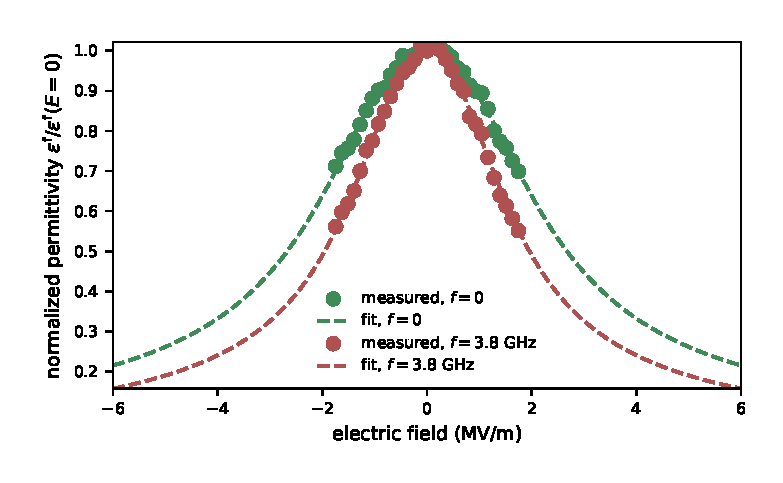
\includegraphics[width=1.\columnwidth]{epsilon_fit}
 \caption{Variation of the ferroelectric permittivity as a function of the
  applied electric field.\vspace*{0.4em}
  \begin{tabular}{llll}
   case        & $\epsf(0)$ & $\alpha$ ($\rm \mu m^2/V^2$) & $\beta$ ($\rm \mu m^4/V^4$) \\ \hline
   static      & 3050       & 0.120                        & 0.024                       \\
   $f=3.8$ GHz & 165        & 0.240                        & 0.079                       \\
  \end{tabular}
  }
 \label{fig1}
\end{figure}


\mysubtitle{Coupled problem}

The electric field $\B E=-\grad V$ derived from the
solution of \equ{eq_elstat} depends on the permittivity distribution, which
itself depends on the electric field through \equ{eq_epsf}.


\end{column}
\end{columns}



\begin{columns}[t,totalwidth=\columnwidth]

\begin{column}{.64\columnwidth}
  \mysubtitle{Homogenization}
  Two scale convergence homogenization \cite{allaire_homogenization_1992, guenneau_homogenization_2000}, TE case:
  solutions $\psi_j$ of two annex problems
  % $\mathcal P_j$, $j=\{1, 2\}$:
  \begin{equation}
   \div \left[ \xitens \grad(\psi_j + r_j) \right] = 0,
   \label{eq_hom_annex}
  \end{equation}
  where $\B r = (x, y)^{\rm T}$ and $\xitens=\epstens^{\rm T}/ {\rm det }(\epstens)$.
  The homogenized tensor $\xihom$ is obtained with:
  \begin{equation}
   \xihom = \langle \xitens \rangle + \B \phi,
   \label{eq_hom}
  \end{equation}
  where $\langle . \rangle$ denotes the mean value over the unit cell.
  Correction terms $\B \phi_{ij} = \langle \xitens \grad \psi_i \rangle_j$.\\
\end{column}

\begin{column}{.3\columnwidth}

  \begin{figure}[!t]
   \centering
   \includegraphics[width=1.\columnwidth]{unit_cell}
   \caption{Periodic unit cell}
   \label{fig_cell}
  \end{figure}

  Effective permittivity tensor: $\epshom=\xihom^{\rm T}/ {\rm det }(\xihom)$.



\end{column}
\end{columns}




\mysubtitle{Open source numerical implementation}
Equations~(\ref{eq_elstat}) and (\ref{eq_hom_annex}) are solved with a Finite Element
Method using the freewares Gmsh \cite{geuzaine_gmsh:_2009} and GetDP \cite{dular_general_1998} driven by a Python package.

\end{posterblock}
\end{textblock*}
%
% %
% %%%%%%%%%%%%% BOX 3 %%%%%%%%%%%%%%%%%%%%%%%%%%%%%%%%%%%%
%
\begin{textblock*}{38.5cm}(2.5cm,80cm)
\begin{posterblock}{Results}{benchcolor1}
 \mysubtitle{Periodic case}
 \begin{figure}[!t]
   \centering
   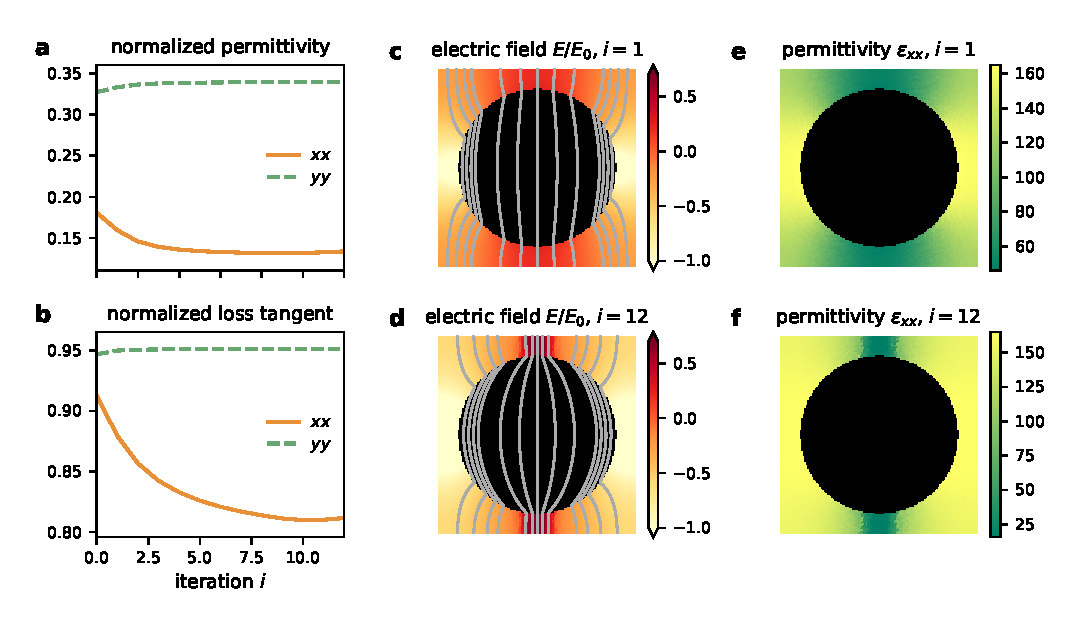
\includegraphics[width=0.9\textwidth]{convergence_per}
   \caption{Convergence of the coupled problem.
    Real part (a) and loss tangent (b) of the components of the homogenized
    permittivity tensor as a function of iteration step $i$. The distribution of
    the normalized electric field (colour map: magnitude in logarithmic scale,
    lines: equipotential contours) and of the
    $xx$ component of the permittivity tensor are shown for $i=1$
    (c and d) and $i=12$ (e and f).
   }
   \label{conv2D}
 \end{figure}
\end{posterblock}

\end{textblock*}
% %
% %
% % %
% % % %%%%%%%%%%%%%%%%%%%%%%%%%%%%%%%%%%%%%%%%%%%%%%%%%%%%%%%%%%%%%%%%%%%%%%%%%%%%
% % %
% % %%%%%%%%%%%%%%%%%%%%%%%%%%%%%%%%%%%%%%%%%%%%%%%%%%%%%%%%%%%%%%%%%%%%%%%%%%%%
% % %%%%%%%%%%% Right column  %%%%%%%%%%%%%%%%%%%%%%%%%%%%%%%%
% % %%%%%%%%%%%%%%%%%%%%%%%%%%%%%%%%%%%%%%%%%%%%%%%%%%%%%%%%%%%%%%%%%%%%%%%%%%%%
% %
% % %%%%%%%%%%%%%%%%%%  BOX %%%%%%%%%%%%%%%%%%%%%%%%%%%%%%%%%%%%%%%%%%%%%%
% %
\begin{textblock*}{38.5cm}(43.5cm,22.5cm)
\begin{posterblock}{Results}{benchcolor1}
  \vspace*{-0.7em}
   \mysubtitle{Effective parameters}
Tunability $n = \varepsilon_{xx}(0)/\varepsilon_{xx}(E)$, anisotropy factor
$a = \varepsilon_{xx}(E)/\varepsilon_{yy}(E)$

\begin{figure}[!t]
 \centering
 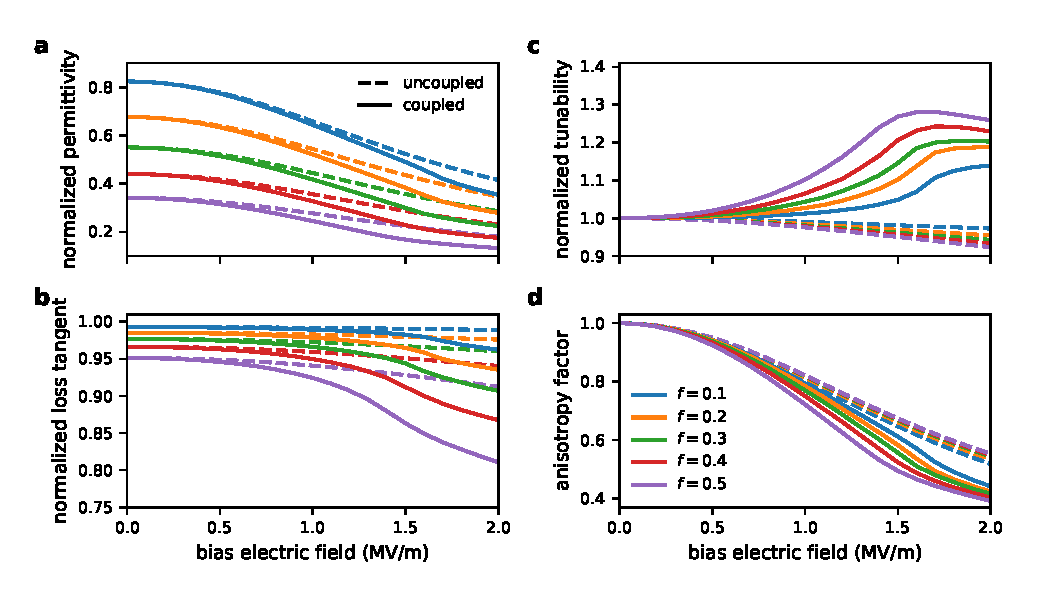
\includegraphics[width=0.9\textwidth]{effective_params_per}
 \caption{Effective parameters of the 2D metamaterials as a function of the
  applied electric field for various filling fraction of dielectric.
  (a): normalized permittivity, (b): normalized loss tangent, (c): normalized tunability and
  (d): anisotropy factor. The solid lines correspond to the coupled model and
  the dashed lines to the uncoupled model. Values are normalized with respect to the bulk properties.}
 \label{eff_par_2D_TM}
\end{figure}

 \mysubtitle{Pseudo-random case}
   \vspace*{-0.7em}
 \begin{figure}[!t]
  \centering
  \includegraphics[width=0.9\textwidth]{rand}
  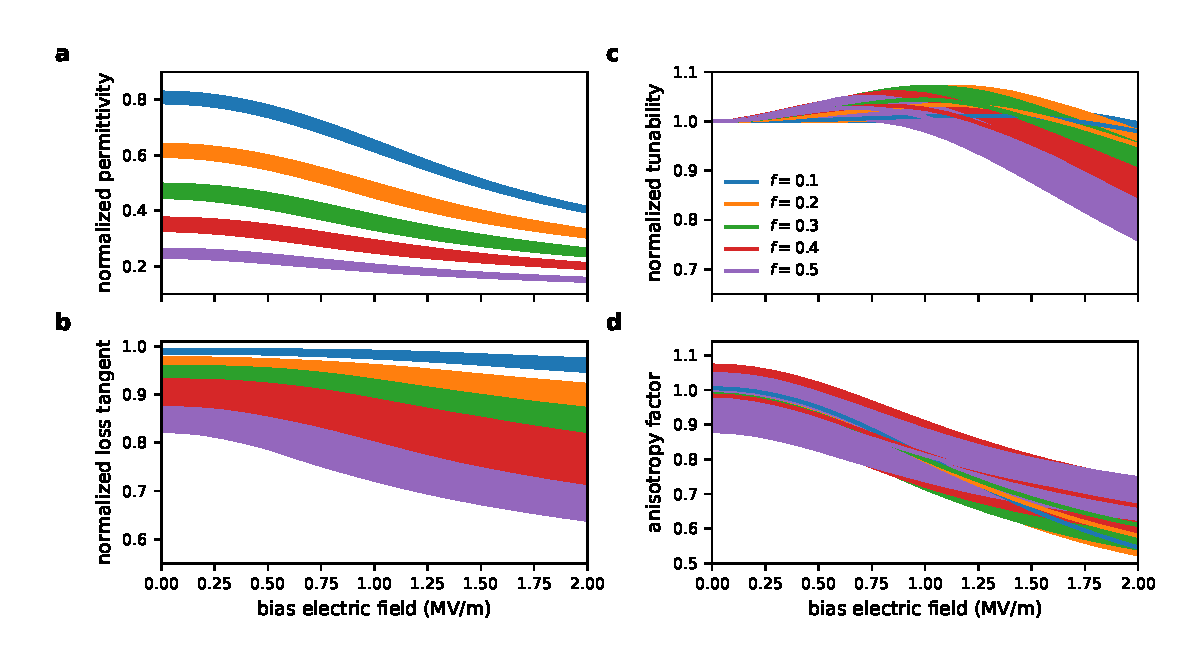
\includegraphics[width=0.9\textwidth]{effpar_rand_cpl}
  \caption{Effective parameters of the pseudo-random composites as a function of the
   applied electric field for various filling fraction of dielectric, when the
   coupling is taken into account.
   (a): normalized permittivity, (b): normalized loss tangent, (c): normalized tunability and
   (d): anisotropy factor. The solid lines represent the average values
   over the 21 samples and the lighter error bands show a confidence interval corresponding to
   the standard deviation.}
  \label{eff_par_2Drand_TM}
 \end{figure}
\end{posterblock}

\end{textblock*}
% % %
% % %
% %%%%%%%%%%%%%%%%%%%%%  Reference box %%%%%%%%%%%%%%%%%%%%%%%%%%%%%%%%%%%%%%%%%
%
\begin{textblock*}{38.5cm}(43.5cm,85.1cm)
\myblocktitle{References}{fresnelgreenblue}
\color{fresnelblack}
\printbibliography
\end{textblock*}

%%%%%%%%%%%%%%%%%%%%%  Acknowledgments box %%%%%%%%%%%%%%%%%%%%%%%%%%%%%%%%%%%%%%%%%
\begin{textblock*}{38.5cm}(43.5cm,105.cm)
\myblocktitle{Acknowledgments}{fresnelgreenblue}
\color{fresnelblack}
This work was funded by the Engineering and Physical Sciences Research
Council (EPSRC), UK, under a grant (EP/P005578/1) 'Adaptive Tools for
Electromagnetics and Materials Modelling to Bridge the Gap between
Design and Manufacturing (AOTOMAT)'
\end{textblock*}
%

\begin{textblock*}{70cm}(12cm,113cm)

{\hfill\semiboldfont \bfseries \color{fresnelorange} \Large CONTACT \& LINKS}\\
\vspace*{0.5em}
\color{white}
\hfill Corresponding author: Benjamin Vial |~\textcolor{fresnelorange}{\href{mailto:b.vial@qmul.ac.uk}{\faEnvelope~b.vial@qmul.ac.uk}}
|~\textcolor{fresnelorange}{\href{http://bvial.info}{\faExternalLink~bvial.info}}\\
\hfill Github |~\textcolor{fresnelorange}{\href{https://github.com/benvial/ferromtm}{\faGithub~github.com/benvial/ferromtm}}\\
\hfill Antennas \& Electromagnetics Research Group |~\textcolor{fresnelorange}{\href{http://antennas.eecs.qmul.ac.uk}{\faExternalLink~antennas.eecs.qmul.ac.uk}}

\end{textblock*}
%% LOGOS %%%%%%%%%%%


\begin{textblock*}{5.5cm}(2.5cm,114cm)
 \includegraphics[width=\columnwidth]{./logos/logo_epsrc.png}
\end{textblock*}

\begin{textblock*}{11cm}(10cm,114cm)
 \includegraphics[width=\columnwidth]{./logos/logo_qmul.png}
\end{textblock*}



\begin{textblock*}{5.5cm}(42.9cm,112.7cm)
 \includegraphics[width=\columnwidth]{./figs/qrcode.png}
\end{textblock*}


%
% \begin{textblock*}{10.8cm}(17.6cm,114cm)
%  \includegraphics[width=\columnwidth]{./logos/logo_qmul.png}%{logo_black.png}
% \end{textblock*}
%
% \begin{textblock*}{8cm}(30.cm,114cm)
%  \includegraphics[width=\columnwidth]{./logos/logo_exeter.png}
% \end{textblock*}
%
% \begin{textblock*}{8.7cm}(39.5cm,114cm)
%  
\includegraphics[width=\columnwidth]{./logos/logo_oxford.png}
% \end{textblock*}



\end{frame}

\end{document}
